\section{Methodology: GDF-Net Architecture and Gradient Decoupling}
\label{sec:method}

In this section, we formulate the mathematical mechanics of recurrent feedback learning, prove the existence of the Feedback Trap in conventional architectures, and present the theoretical derivation and architectural components of our proposed \textbf{GDF-Net} (Gradient-Decoupled Feedback Network) equipped with the \textbf{Multi-Scale Gradient-Decoupled Feedback Decoder}.

% -----------------------------------------------------------------------------
\subsection{The Classical Feedback Formulation and the Feedback Trap}
In classical recurrent feedback vision networks, an image $\mathbf{x} \in \mathbb{R}^{B \times 3 \times H \times W}$ is processed iteratively across feedback time-steps $t \in \{1, \dots, T\}$. At step $t=1$, the network operates in an initial feedforward pass with no prior prediction ($m^{(0)} = \mathbf{0}$), generating an initial segmentation probability map $m^{(1)} = \sigma(\hat{y}^{(1)})$. At step $t > 1$, the previous prediction $m^{(t-1)}$ is recursively reinjected into the network layers to guide subsequent feature extraction.

In conventional recurrent feedback designs, this recurrent fusion is typically executed via hard spatial gating or max-pooling operators. Within intermediate encoder and decoder stages, an input feature tensor $\mathbf{F} \in \mathbb{R}^{B \times C \times H' \times W'}$ is processed by an internal convolutional attention branch $\mathcal{F}_{\text{att}}$, producing an attention map $\text{fmask} \in [0, 1]^{B \times 1 \times H' \times W'}$. Simultaneously, the recurrent mask $m^{(t-1)}$ is downsampled to spatial resolution $(H', W')$, yielding $m_{\text{fg}}$. These two spatial signals are fused through a hard binary thresholding operator:
\begin{equation}
  \label{eq:keep_hard}
  \text{keep}_{\text{hard}} = \max\!\left(\mathbb{I}(\text{fmask} > 0.5),\; m_{\text{fg}}\right),
\end{equation}
which gates the feature representations prior to downstream processing.

\subsubsection{Mathematical Proof of Gradient Paralysis}
\begin{theorem}[Gradient Paralysis of Internal Attention]
Let $\mathcal{L}$ be any differentiable segmentation loss function, and let features be gated by $\text{keep}_{\text{hard}}$ defined in Eq.~(\ref{eq:keep_hard}). The gradient of $\mathcal{L}$ with respect to the parameters $\theta_{\text{att}}$ of the attention generator $\mathcal{F}_{\text{att}}$ is zero almost everywhere:
\begin{equation}
  \frac{\partial \mathcal{L}}{\partial \theta_{\text{att}}} \equiv 0 \quad \text{almost everywhere}.
\end{equation}
\end{theorem}

\begin{proof}
By applying the multivariate chain rule across the gated feature path:
\begin{equation}
  \label{eq:chain_rule}
  \frac{\partial \mathcal{L}}{\partial \theta_{\text{att}}} = \frac{\partial \mathcal{L}}{\partial \mathbf{F}_{\text{gated}}} \cdot \frac{\partial \mathbf{F}_{\text{gated}}}{\partial \text{keep}_{\text{hard}}} \cdot \frac{\partial \text{keep}_{\text{hard}}}{\partial \text{fmask}} \cdot \frac{\partial \text{fmask}}{\partial \theta_{\text{att}}}.
\end{equation}
The term $\text{keep}_{\text{hard}}$ utilizes the indicator step function $\mathbb{I}(\text{fmask} > 0.5)$. The distributional derivative of the Heaviside step function is the Dirac delta function $\delta(u - 0.5)$, which vanishes for all inputs $u \neq 0.5$:
\begin{equation}
  \frac{\partial}{\partial u}\mathbb{I}(u > 0.5) = 0 \quad \forall\, u \in \mathbb{R} \setminus \{0.5\}.
\end{equation}
Consequently, $\frac{\partial \text{keep}_{\text{hard}}}{\partial \text{fmask}} = 0$ on the support of continuous activations. Substituting into Eq.~(\ref{eq:chain_rule}) yields $\frac{\partial \mathcal{L}}{\partial \theta_{\text{att}}} \equiv 0$ almost everywhere.
\end{proof}

\textbf{Consequence:} The learnable convolutional layers dedicated to extracting internal spatial attention receive zero direct supervision from the segmentation objective. The attention mechanism remains virtually frozen at its random initialization.

\subsubsection{Unconstrained Recursive Backpropagation and Error Amplification}
While the internal attention branch receives zero gradient, automatic differentiation propagates non-zero gradients freely through the recurrent mask branch:
\begin{equation}
  \frac{\partial \mathcal{L}}{\partial m_{\text{fg}}} = \frac{\partial \mathcal{L}}{\partial \mathbf{F}_{\text{gated}}} \cdot \frac{\partial \mathbf{F}_{\text{gated}}}{\partial \text{keep}_{\text{hard}}} \cdot \frac{\partial \text{keep}_{\text{hard}}}{\partial m_{\text{fg}}} \neq 0.
\end{equation}
Because prediction $m^{(t-1)}$ is a direct function of encoder-decoder parameters $\Theta$, backpropagating through $m_{\text{fg}}$ creates an unconstrained recursive dependency:
\begin{equation}
  \nabla_\Theta \mathcal{L}^{(t)} = \frac{\partial \mathcal{L}^{(t)}}{\partial \hat{y}^{(t)}} \left[ \frac{\partial \hat{y}^{(t)}}{\partial \Theta} + \frac{\partial \hat{y}^{(t)}}{\partial m^{(t-1)}} \cdot \frac{\partial m^{(t-1)}}{\partial \Theta} \right].
\end{equation}
When the network generates a false positive at step $t-1$, that error is injected into the forward pass. In the backward pass, the second term forces the encoder to optimize for consistency with past errors rather than anatomical truth. This causes catastrophic Batch Normalization drift, shifts intermediate feature representations, and locks the model into an irreversible cycle of false-positive over-segmentation (the \textit{Feedback Trap}).

% -----------------------------------------------------------------------------
\subsection{The Feedback Firewall Principle (Gradient Decoupling)}
To resolve the Feedback Trap, we establish the \textbf{Feedback Firewall} principle:
\begin{center}
  \textit{Forward prediction history must provide spatial guidance without permitting backward recursive gradient propagation.}
\end{center}
Mathematically, we introduce the stop-gradient operator $\text{detach}(\cdot)$ at the feedback boundary:
\begin{equation}
  \mathbf{m}_{\text{guide}} = \text{detach}\left(m^{(t-1)}\right), \quad \text{where} \quad \frac{\partial \mathbf{m}_{\text{guide}}}{\partial \Theta} \equiv 0.
\end{equation}
Under this operator, the gradient of the recurrent step simplifies strictly to:
\begin{equation}
  \nabla_\Theta \mathcal{L}^{(t)} = \frac{\partial \mathcal{L}^{(t)}}{\partial \hat{y}^{(t)}} \cdot \left. \frac{\partial \hat{y}^{(t)}}{\partial \Theta} \right|_{\mathbf{m}_{\text{guide}} = \text{const}}.
\end{equation}
The recurrent feedback now acts strictly as an exogenous spatial prior conditioning the feature distribution, completely severing the recursive gradient feedback loop and eliminating error amplification.

% -----------------------------------------------------------------------------
\subsection{Architecture of GDF-Net}
Building upon the Feedback Firewall principle, we construct \textbf{GDF-Net} (Gradient-Decoupled Feedback Network). The architecture comprises three integrated components: (1) a 4-channel decoupled guidance stem, (2) a pre-trained ResNet-34 encoder backbone, and (3) a Multi-scale Gradient-Decoupled Feedback Decoder, as illustrated in Fig.~\ref{fig:architecture}.

\begin{figure*}[t!]
\centering
\begin{subfigure}[b]{0.48\textwidth}
  \centering
  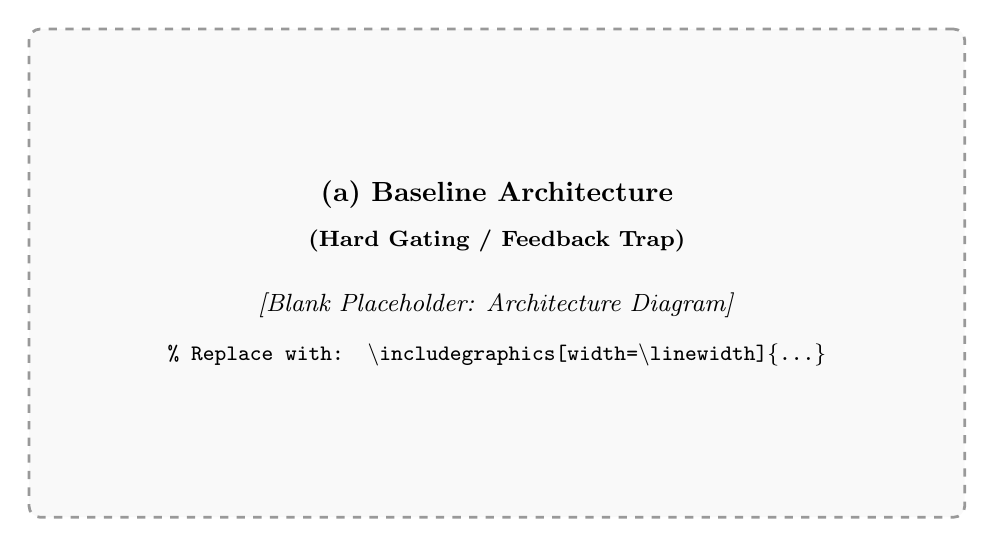
\begin{tikzpicture}
    \node[draw=black!40, dashed, fill=gray!5, rounded corners=4pt, line width=1pt, minimum width=0.98\linewidth, minimum height=6.2cm, align=center] {
      \textbf{\normalsize (a) Baseline Architecture}\\[1.5mm]
      \textbf{\footnotesize (Hard Gating / Feedback Trap)}\\[4mm]
      \textit{\small [Blank Placeholder: Architecture Diagram]}\\[2mm]
      {\footnotesize \texttt{\% Replace with: \textbackslash includegraphics[width=\textbackslash linewidth]\{...\}}}
    };
  \end{tikzpicture}
  \caption{Baseline Architecture}
  \label{fig:arch_baseline}
\end{subfigure}
\hfill
\begin{subfigure}[b]{0.48\textwidth}
  \centering
  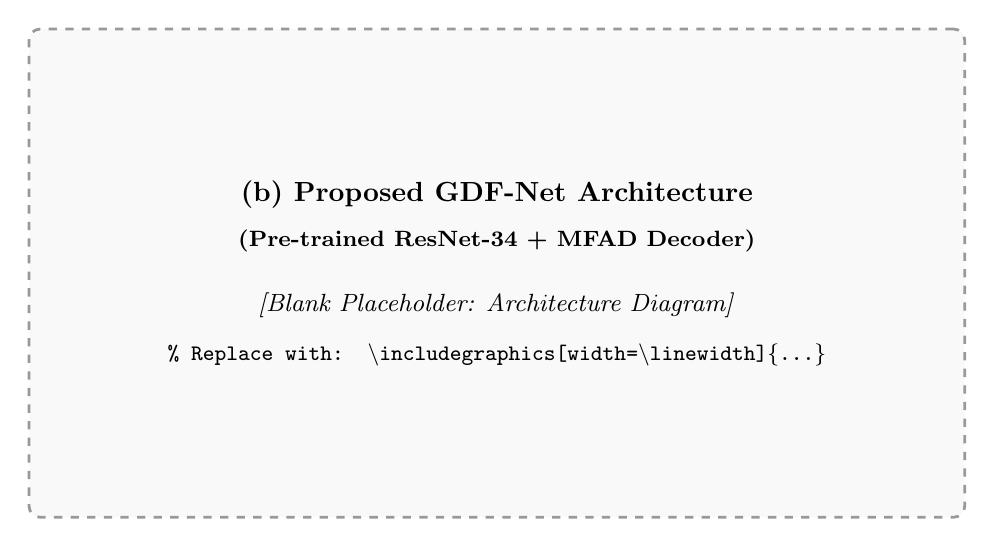
\begin{tikzpicture}
    \node[draw=black!40, dashed, fill=gray!5, rounded corners=4pt, line width=1pt, minimum width=0.98\linewidth, minimum height=6.2cm, align=center] {
      \textbf{\normalsize (b) Proposed GDF-Net Architecture}\\[1.5mm]
      \textbf{\footnotesize (Pre-trained ResNet-34 + MFAD Decoder)}\\[4mm]
      \textit{\small [Blank Placeholder: Architecture Diagram]}\\[2mm]
      {\footnotesize \texttt{\% Replace with: \textbackslash includegraphics[width=\textbackslash linewidth]\{...\}}}
    };
  \end{tikzpicture}
  \caption{Proposed GDF-Net Architecture (Ours)}
  \label{fig:arch_proposed}
\end{subfigure}
\caption{Architectural comparison between the coupled baseline and the proposed Gradient-Decoupled Feedback Network (\textbf{GDF-Net}). \textbf{(a) Baseline Architecture (Hard Gating / Feedback Trap):} Relies on a custom 4-stage convolutional encoder trained from scratch. The non-differentiable indicator gating ($\mathbb{I}(f_{\text{mask}} > 0.5)$) induces complete gradient paralysis ($\nabla_{f_{\text{mask}}} \equiv 0$), while unconstrained recursive backpropagation across feedback steps ($t=1 \to t=2$) injects past prediction errors into internal representations, triggering catastrophic Batch Normalization drift and irreversible false-positive expansion. \textbf{(b) Proposed GDF-Net Architecture (Ours):} Employs a pre-trained ResNet-34 transfer backbone accepting a 4-channel input stem, where the detached spatial prior ($m^{(t-1)}.\text{detach}()$) is adaptively modulated by a learned spatial gate. The Feedback Firewall strictly eliminates backward recursive gradient dependencies ($\nabla_{m^{(t-1)}} \equiv 0$), while the Multi-Scale Feedback Attention Decoder (\textbf{MFAD}) provides smooth, non-zero gradient modulation ($\mathbf{F} \odot (1.0 + \text{Att}(m))$) across all five hierarchical decoder scales, ensuring stable training convergence, robust false-positive suppression, and sharp anatomical boundary refinement.}
\label{fig:architecture}
\label{fig:architecture_diagram}
\end{figure*}


\subsubsection{4-Channel Decoupled Guidance Stem}
At feedback step $t$, the detached mask prior $\mathbf{m}_{\text{guide}} \in [0, 1]^{B \times 1 \times H \times W}$ is first modulated by a learned $1 \times 1$ spatial convolutional gate $\mathcal{W}_{\text{gate}}$:
\begin{equation}
  \mathbf{x}_{\text{guide}} = \sigma\left(\mathcal{W}_{\text{gate}} * \mathbf{m}_{\text{guide}}\right).
\end{equation}
The modulated guidance is concatenated directly with the raw RGB image $\mathbf{x}_{\text{RGB}} \in \mathbb{R}^{B \times 3 \times H \times W}$ along the channel dimension to form a 4-channel input tensor:
\begin{equation}
  \mathbf{x}_{\text{in}} = \left[\mathbf{x}_{\text{RGB}} \,\|\, \mathbf{x}_{\text{guide}}\right] \in \mathbb{R}^{B \times 4 \times H \times W}.
\end{equation}
The stem convolution $\text{Conv}_{7 \times 7}$ accepts 4 input channels. We initialize the first 3 channels with pre-trained ImageNet weights from ResNet-34, while the 4th channel is initialized with zeros, ensuring stable warm-up during early iterations:
\begin{equation}
  \mathcal{W}_{\text{stem}}[:, 0:3, :, :] = \mathcal{W}_{\text{ResNet}}, \quad \mathcal{W}_{\text{stem}}[:, 3, :, :] = 0.
\end{equation}

\subsubsection{Hierarchical Encoder Backbone}
Features are extracted using a standard ResNet-34 backbone~\cite{he2016deep}, yielding five hierarchical feature representations:
\begin{align}
  \mathbf{e}_1 &\in \mathbb{R}^{B \times 64 \times \frac{H}{2} \times \frac{W}{2}}, \quad
  \mathbf{e}_2 \in \mathbb{R}^{B \times 64 \times \frac{H}{4} \times \frac{W}{4}}, \\
  \mathbf{e}_3 &\in \mathbb{R}^{B \times 128 \times \frac{H}{8} \times \frac{W}{8}}, \quad
  \mathbf{e}_4 \in \mathbb{R}^{B \times 256 \times \frac{H}{16} \times \frac{W}{16}},
\end{align}
\begin{equation}
  \mathbf{b} \in \mathbb{R}^{B \times 512 \times \frac{H}{32} \times \frac{W}{32}}.
\end{equation}

\subsubsection{Multi-Scale Gradient-Decoupled Feedback Decoder}
Unlike conventional feedback designs that restrict recurrent gating to isolated bottleneck layers or single stages, our proposed multi-scale decoder integrates continuous spatial modulation across all five hierarchical decoder levels $\ell \in \{1, 2, 3, 4, 5\}$.

At each decoder level $\ell$, intermediate encoder skip-connection features $\mathbf{e}_\ell$ are modulated by the detached spatial prior $\mathbf{m}_{\text{guide}}$. First, $\mathbf{m}_{\text{guide}}$ is adaptively interpolated via bilinear sampling to match the spatial resolution $(H_\ell, W_\ell)$ of feature map $\mathbf{e}_\ell$:
\begin{equation}
  \mathbf{m}_\ell = \text{BilinearInterpolate}\left(\mathbf{m}_{\text{guide}}, (H_\ell, W_\ell)\right).
\end{equation}
A dedicated attention submodule $\mathcal{A}_\ell$ generates a continuous spatial weight map:
\begin{equation}
  \mathbf{S}_\ell = \sigma\left(\text{BN}\left(\text{Conv}_{1 \times 1}\left(\mathbf{m}_\ell\right)\right)\right) \in (0, 1)^{B \times C_\ell \times H_\ell \times W_\ell}.
\end{equation}
Features are modulated via a residual multiplicative attention gate:
\begin{equation}
  \label{eq:gdf_modulation}
  \mathbf{e}_{\ell, \text{guided}} = \mathbf{e}_\ell \odot \left(1.0 + \mathbf{S}_\ell\right).
\end{equation}
Equation~(\ref{eq:gdf_modulation}) guarantees three vital mathematical properties:
\begin{enumerate}
  \item \textbf{Identity Preservation:} When prior guidance is absent or uninformative ($\mathbf{S}_\ell \to 0$), the feature reduces smoothly to the original representation $\mathbf{e}_\ell$, preventing signal attenuation.
  \item \textbf{Dense Gradient Flow:} Unlike the discontinuous indicator function in Eq.~(\ref{eq:keep_hard}), Eq.~(\ref{eq:gdf_modulation}) is smooth and continuously differentiable everywhere:
  \begin{equation}
    \frac{\partial \mathbf{e}_{\ell, \text{guided}}}{\partial \mathbf{e}_\ell} = 1.0 + \mathbf{S}_\ell \ge 1.0,
  \end{equation}
  guaranteeing robust gradient backpropagation throughout the decoder and skip pathways.
  \item \textbf{Multi-Resolution Refinement:} By operating from coarse bottleneck scale ($H/32$) up to full feature resolution ($H/2$), the GDF Decoder provides contextual constraints across both semantic localization and fine boundary contours.
\end{enumerate}

Each decoder stage synthesizes features via a transposed convolution followed by dual $3 \times 3$ convolutional blocks with Batch Normalization and ReLU activations:
\begin{equation}
  \mathbf{d}_\ell = \text{ConvBlock}\left(\left[\text{ConvTranspose}(\mathbf{d}_{\ell-1}) \,\|\, \mathbf{e}_{\ell, \text{guided}}\right]\right).
\end{equation}
The final output is projected via a $1 \times 1$ convolution to generate logit map $\hat{y}^{(t)} \in \mathbb{R}^{B \times 1 \times H \times W}$.

% -----------------------------------------------------------------------------
\subsection{Training Objective and Multi-Pass Optimization}
The network is optimized using a compound loss function balancing region overlap and pixel-wise probability calibration:
\begin{equation}
  \mathcal{L}_{\text{total}} = 0.5 \cdot \mathcal{L}_{\text{BCE}}\left(\hat{y}, y\right) + 0.5 \cdot \mathcal{L}_{\text{Dice}}\left(\hat{y}, y\right),
\end{equation}
where $\mathcal{L}_{\text{BCE}}$ is binary cross-entropy with logits and $\mathcal{L}_{\text{Dice}}$ is defined with Laplace smoothing $\epsilon = 10^{-5}$:
\begin{equation}
  \mathcal{L}_{\text{Dice}}\left(\hat{y}, y\right) = 1.0 - \frac{2 \sum_i p_i y_i + \epsilon}{\sum_i p_i + \sum_i y_i + \epsilon}, \quad p_i = \sigma(\hat{y}_i).
\end{equation}
During training, each batch undergoes dual forward-backward passes ($T=2$). The initial pass computes $\hat{y}^{(1)} = \mathcal{M}(\mathbf{x}, \emptyset)$, and the second pass computes $\hat{y}^{(2)} = \mathcal{M}(\mathbf{x}, \sigma(\hat{y}^{(1)}))$. Backward optimization is performed on the final prediction $\hat{y}^{(2)}$, enforcing the decoupled feedback loop.
